\def\QRCODE{MASTER_mispa_TUT.IMG.image_segmentation_watershed_pythonqrcode.png}
\def\QRPAGE{http://www.iptutorials.science/tree/master/MASTER_mispa/TUT.IMG.image_segmentation_watershed/python}
\pcorrectionsection{Python correction}

\begin{python}
import numpy as np
from scipy import misc
import matplotlib.pyplot as plt
from scipy import ndimage as ndi
from scipy.ndimage.morphology import distance_transform_edt
from scipy.ndimage.morphology import distance_transform_cdt
from skimage import morphology
\end{python}


\vspace*{-8pt}

\subsection{Watershed and distance map}
\subsubsection{Regional maxima}
The following code is an implementation of the regional maxima (from mathematical morphology definition). It deals with the case of float images as input.
\begin{python}
def rmax(I):    
    """
    Own version of regional maximum
    This avoids plateaus problems of peak_local_max
    I: original image, int values
    returns: binary array, with True for the maxima
    """
    I = I.astype('float');
    I = I / np.max(I) * 2**31;
    I = I.astype('int32');
    h = 1;
    rec = morphology.reconstruction(I, I+h);
    maxima = I + h - rec;
    return maxima>0
\end{python}

\subsubsection{Distance map followed by a watershed}
This method is a classical way of performing the separation of some objects by proximity or influence zones. It is illustrated in Fig.\ref{fig:watershed:python:dm}.

\begin{python}
A = imageio.imread('circles.tif');
# chamfer distance gives integer distances
dm = distance_transform_edt(A);
# regional maxima
local_maxi = rmax(dm);
\end{python}
The local maxima will be used as a marker for the watershed operation, in order to perform the separation of the grains, see Fig.\ref{fig:watershed:python:dm}.
\begin{python}
# watershed segmentation for separating the circles
markers = ndi.label(local_maxi, np.ones((3, 3)))[0]
W = morphology.watershed(-dm, markers, watershed_line=True)
# separation of the grains
B = A & W==0;
separation = ndi.label(B, np.ones((3,3)))[0];
\end{python}

\begin{figure}[H]
 \centering\caption{Steps of the separation of the grains.}%
 \subfloat[Original image.]{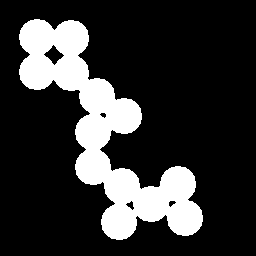
\includegraphics[width=.3\linewidth]{circles.png}}\hfill
 \subfloat[Distance map.]{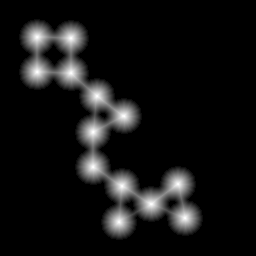
\includegraphics[width=.3\linewidth]{dm.python.png}}\hfill
 \subfloat[Separation of the grains.]{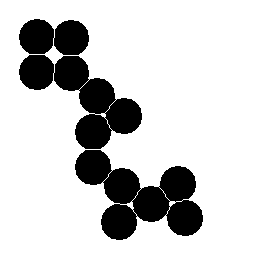
\includegraphics[width=.3\linewidth]{separation.python.png}}%
 \label{fig:watershed:python:dm}%
 \vspace*{-10pt}%
\end{figure}

\vspace*{-15pt}

\subsection{Watershed and image gradients}
The gradient image amplifies the noise. Thus, the watershed operator directly applied to the gradient of the image produces an over-segmented image (see Fig.\ref{fig:watershed:python:wat}).

\begin{python}
def sobel_mag(im):
    """
    Returns Sobel gradient magnitude
    im: image array of type float
    returns: magnitude of gradient (L2 norm)
    """
    dx = ndi.sobel(im, axis=1)   # horizontal derivative
    dy = ndi.sobel(im, axis=0)   # vertical derivative
    mag = np.hypot(dx, dy)  # magnitude
    return mag;
\end{python}

\vspace*{-8pt}

\begin{figure}[H]
 \centering\caption{Performing the watershed on the gradient image is usually not a good idea.}%
 \subfloat[Original image.]{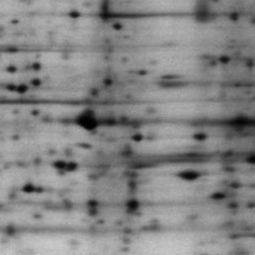
\includegraphics[width=.3\linewidth]{gel.jpg}}\hfill
 \subfloat[{\textls[-50]{Amplitude of the gradient (Sobel).}}]{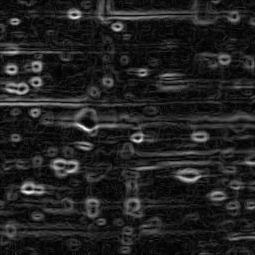
\includegraphics[width=.3\linewidth]{sobel.python.png}}\hfill
 \subfloat[Watershed segmentation.]{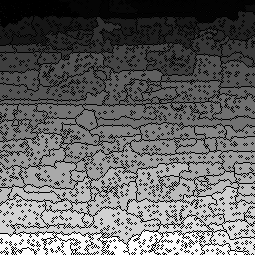
\includegraphics[width=.3\linewidth]{gel_gradient.python.png}}%
  \vspace*{-10pt}%
 \label{fig:watershed:python:wat}%
\end{figure}

\vspace*{-10pt}

In fact, this method produces as many segments as there are minima in the gradient image Fig.\ref{fig:watershed:python:minima}.

\vspace*{-8pt}

\begin{figure}[H]
\centering\caption{Local minima of the gradient image.}%
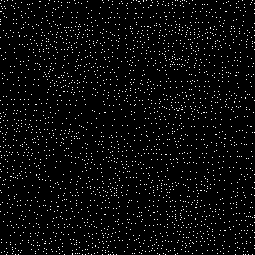
\includegraphics[width=.25\linewidth]{markers_gel.python.png}%
 \label{fig:watershed:python:minima}%
\end{figure}

\subsubsection{Solution: filtering the image}
Before evaluating the gradient, the image is filtered. The number of minima is lower and this leads to a less over-segmented image (Fig.\ref{fig:watershed:python:wat_filtered}).

\begin{python}
SE = morphology.disk(2);
O = morphology.opening(gel, selem=SE);
F = morphology.closing(O,   selem=SE).astype('float');
g = sobel_mag(F).astype('float');
\end{python}

\vspace*{-8pt}

\begin{figure}[htbp]
 \centering\caption{Even if the gradient is performed on the filtered image, there is still a high over-segmentation.}%
 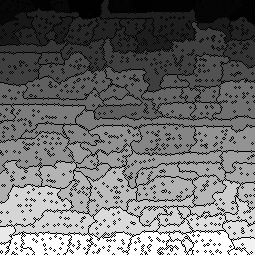
\includegraphics[width=.28\linewidth]{gel_gradient_filtered.python.png}%
 \label{fig:watershed:python:wat_filtered}%
\end{figure}

\vspace*{-15pt}

\subsection{Watershed constrained by markers}
The watershed can be constrained by markers: the markers can provide the correct number of regions. This method imposes both the background
(external markers) and the objects (internal markers). The results are illustrated in Fig.\ref{fig:watershed:python:constrained}.
The ultimate erosion of the internal markers is used to deconnect these markers from the external markers.

\begin{python}
local_maxi = rmax(255-F);
markers = ndi.label(local_maxi, np.ones((3, 3)))[0]
W = morphology.watershed(F, markers, watershed_line=True)

markers2 = local_maxi | (W==0);
M = ndi.label(markers2, np.ones((3, 3)))[0]
segmentation = morphology.watershed(g, M, watershed_line=True);

gel[segmentation==0] = 255;
plt.imshow(gel);
plt.show();
imageio.imwrite("segmentation.python.png", gel);
\end{python}

\vspace*{-10pt}

\begin{figure}[H]
 \centering\caption{Watershed segmentation by markers.}%
 \subfloat[Markers of the background and of the objects.]{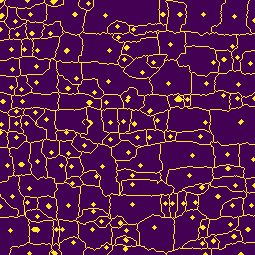
\includegraphics[width=.28\linewidth]{markers_filtered.python.png}} \hspace{1cm}
 \subfloat[Final seg\-men\-ta\-tion.]{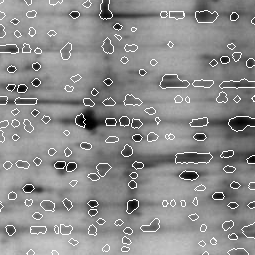
\includegraphics[width=.28\linewidth]{segmentation.python.png}}%
 \label{fig:watershed:python:constrained}%
 \vspace*{-10pt}%
\end{figure}